% This is samplepaper.tex, a sample chapter demonstrating the
% LLNCS macro package for Springer Computer Science proceedings;
% Version 2.20 of 2017/10/04
%
\documentclass[12pt]{article}
%
\usepackage{graphicx}
% \usepackage[latin1]{inputenc}
\usepackage[british]{babel}
\usepackage[all]{xy}
\usepackage{amscd}
\usepackage{amssymb}
\usepackage{amsthm}
\usepackage{enumitem}
\usepackage{mathrsfs,bbm}
\usepackage{xcolor,graphicx}
\usepackage{graphics}
\usepackage{soul}
\usepackage{comment}
\usepackage[all]{xy}
\usepackage{amscd}
\usepackage{amssymb,amsmath,latexsym}
\usepackage{amsthm}
\usepackage{enumitem}
\usepackage{mathrsfs,bbm}
\usepackage{dsfont}
\usepackage{tikz-cd}
\usepackage[T1]{fontenc}
\usepackage[utf8]{inputenc}  
 %
%%%%%%%%%%%%%%%%%%%%%%%%%%%%%%%%%%
%pagestyle
%%%%%%%%%%%%%%%%%%%%%%%%%%%%%%%%%%
%\pagestyle{plain}
\textwidth=430pt
\headsep=.7cm
\evensidemargin=15pt
\oddsidemargin=15pt
\leftmargin=0cm
\rightmargin=0cm
%%
%%%%%%%%%%%%%%%%%%%%%%%
\newcommand*\fixitem {\item[]%
  \refstepcounter{enumi}\hskip-\leftmargin\labelenumi\hskip\labelsep}
\newtheorem*{mainthm}{Main Theorem}
\newtheorem*{mainthm1}{Theorem}
\newtheorem*{maincor}{Corollary}
\usepackage[colorlinks=true]{hyperref}
\DeclareMathOperator{\Forall}{\forall}
\DeclareMathOperator{\Exists}{\exists}
\DeclareMathOperator{\ord}{ord}
\newcommand{\phiD}{\varphi_D}
\newcommand{\phiDI}{\varphi_{\mathbf{D}_I}}
\newcommand{\phiDIj}{\varphi_{\mathbf{D}_I (j)}}
\newcommand{\phiH}{\varphi_H}
\newcommand{\phiTimes}{\phiD \otimes \phiH}
\newcommand{\phiTimesDI}{\varphi_{\mathbf{D}_I} \otimes \phiH}
\newcommand{\R}{\mathscr{A}}
\newcommand{\X}{\mathscr{X}}
\newcommand{\Xf}{\mathscr{X}_{(k_0 ,i)}[r_0]}
\newcommand{\Xfr}{\mathscr{X}_{(k_0,i)}[r]}
\newcommand{\hotimes}{\widehat{\otimes}}
\newcommand{\C}{\mathbb{C}_p}
\newcommand{\V}{\mathscr{V}}
\newcommand{\B}{\mathscr{B}}
\newcommand{\dualD}{\mathfrak{D}}
\newcommand{\Dg}{\mathbf{D}}
\newcommand{\DD}{\mathcal{D}^0}
\newcommand{\DDg}{\mathcal{D}}
\newcommand{\DV}{\mathcal{D}}
\newcommand{\W}{\mathscr{W}_N}
\newcommand{\Ao}{\mathbf{A}^\circ}
\newcommand{\AoK}{\mathbf{A}^\circ_{\K}}
\newcommand{\AK}{\mathbf{A}_{/\K}}
\newcommand{\OOO}{\mathscr{A}^\circ}
\newcommand{\K}{\mathcal{K}} 
\newcommand{\OK}{\mathcal{O}_{\K}}
\newcommand{\varprojlog}[1]{\underleftarrow{\log\!^{#1}}}
\newcommand{\T}{\mathscr{T}}
\newcommand{\TT}{\mathbf{T}}
\newcommand{\VV}{\mathbf{V}}
\newcommand{\HH}{\mathcal{H}}
\newcommand{\hh}{\mathcal{H}^+}
\newcommand{\HG}[2]{\mathcal{H}_{#1}(#2)}
\newcommand{\hhl}{\mathcal{H}^{+,[l]}}
\newcommand{\hhj}{\mathcal{H}^{+,[j]}}
\newcommand{\hhjj}{\mathcal{H}^{+,[l,l']}}
\newcommand{\GS}{G_{\mathbb{Q},S}}
\newcommand{\Rf}{R_{(k_0 ,i)}[r_0]}
\newcommand{\Rfr}{R_{(k_0 ,i)}[r]}
\newcommand{\parT}{\langle T\rangle}
\newcommand{\Zf}{Z_{(k_0 ,i)}[r_0]}
\newcommand{\Zfr}{\mathscr{Z}_{(k_0 ,i)}[r]}
\newcommand{\ZFf}{\mathscr{Z}_{(k_0 ,i)}[r_0]}
\newcommand{\ZFfr}{\mathscr{Z}_{(k_0 ,i)}[r]}
\newcommand{\ZF}{\mathscr{Z}}
% Used for displaying a sample figure. If possible, figure files should
% be included in EPS format.
%
% If you use the hyperref package, please uncomment the following line
% to display URLs in blue roman font according to Springer's eBook style:
 \renewcommand\UrlFont{\color{blue}\rmfamily}

\begin{document}
%
\title{Efficient Symbolic Reasoning for Neural-Network Verification}
\date{}
%
%\titlerunning{Abbreviated paper title}
% If the paper title is too long for the running head, you can set
% an abbreviated paper title here
%
\author{\small Zi Wang$^{\dag}$  \;\;   Somesh Jha$^{\dag}$\;\; Krishnamurthy (Dj) Dvijotham$^{\ddag}$ \; \\$^{\dag}$\small University of Wisconsin-Madison 
\; $^{\ddag}$Google Research\\\texttt{\small zw@cs.wisc.edu, jha@cs.wisc.edu, dvij@google.com}  }
\date{}
%
%\authorrunning{F. Author et al.}
% First names are abbreviated in the running head.
% If there are more than two authors, 'et al.' is used.
%
%\institute{Princeton University, Princeton NJ 08544, USA \and
%Springer Heidelberg, Tiergartenstr. 17, 69121 Heidelberg, Germany
%\email{lncs@springer.com}\\
%\url{http://www.springer.com/gp/computer-science/lncs} \and
%ABC Institute, Rupert-Karls-University Heidelberg, Heidelberg, Germany\\
%\email{\{abc,lncs\}@uni-heidelberg.de}}
%
\maketitle              % typeset the header of the contribution
%
%
%
%


Over the past few years, there has been a significant amount of research focused on studying the ReLU activation function, with the aim of achieving neural network convergence through over-parametrization. However, recent developments in the field of Large Language Models (LLMs) have sparked interest in the use of exponential activation functions, specifically in the attention mechanism.

Mathematically, we define the neural function $F: \R^{d \times m} \times  \mathbb{R}^d \rightarrow \mathbb{R}$ using an exponential activation function. Given a set of data points with labels $\{(x_1, y_1), (x_2, y_2), \dots, (x_n, y_n)\} \subset \mathbb{R}^d \times \mathbb{R}$ where $n$ denotes the number of the data. Here $F(W(t),x)$ can be expressed as $F(W(t),x) := \sum_{r=1}^m a_r \exp(\langle w_r, x \rangle)$, where $m$ represents the number of neurons, and $w_r(t)$ are weights at time $t$. It's standard in literature that $a_r$ are the fixed weights and it's never changed during the training. We initialize the weights $W(0) \in \mathbb{R}^{d \times m}$ with random Gaussian distributions, such that $w_r(0) \sim \mathcal{N}(0, I_d)$ and initialize $a_r$ from random sign distribution for each $r \in [m]$.

Using the gradient descent algorithm, we can find a weight $W(T)$ such that $\| F(W(T), X) - y \|_2 \leq \epsilon$ holds with probability $1-\delta$, where $\epsilon \in (0,0.1)$ and $m = \Omega(n^{2+o(1)}\log(n/\delta))$. To optimize the over-parametrization bound $m$, we employ several tight analysis techniques from previous studies [Song and Yang arXiv 2019, Munteanu, Omlor, Song and Woodruff ICML 2022]. 

 

\section{Introduction}
\label{sec:introduction}
% \begin{itemize}
%     % Diffusion of FL
%     \item {\st{Diffusion of FL}}
%     % Security threats to FL
%     \item {\st{Security threats to FL with particular focus on model poisoning}}
%     % Limitations of existing countermeasures
%     \item {\st{Current countermeasures (e.g., KRUM) and their limitations}}
%     % Proposed method and its advantages
%     \item {\st{Intuitive description of the proposed method and its difference (i.e., advantages) w.r.t. state of the art}}
%     % Main contributions
%     \item {\st{Summary of the main contributions of this work}}
%     % Paper's structure and organization
%     \item {\st{Paper's structure and organization}}
% \end{itemize}

% Diffusion of FL
Recently, {\em federated learning} (FL) has emerged as the leading paradigm for training distributed, large-scale, and privacy-preserving machine learning (ML) systems~\cite{mcmahan2017googleai,mcmahan2017aistats}. 
The core idea of FL is to allow multiple edge clients to collaboratively train a shared, global model without disclosing their local private training data.
%Specifically, an FL system consists of a central server and many edge clients; 
A typical FL round involves the following steps: {\em(i)} the server randomly picks some clients and sends them the current, global model; {\em(ii)} each selected client locally trains its model with its own private data; then, it sends the resulting local model to the server;\footnote{Whenever we refer to global/local model, we mean global/local model {\em parameters}.} {\em(iii)} the server updates the global model by computing an \emph{aggregation function}, usually the average (FedAvg), on the local models received from clients.
% \begin{enumerate}
%     \item[{\em(i)}] the server sends the current, global model to the clients and appoints some of them for training;
%     \item[{\em(ii)}] each selected client locally trains its copy of the global model with its own private data; then, it sends the resulting local model back to the server;\footnote{Whenever we refer to global/local model, we mean global/local model {\em parameters}.}
%     \item[{\em(iii)}] the server updates the global model by computing an \emph{aggregation function} on the local models received from clients (by default, the average, also referred to as FedAvg~\cite{mcmahan2017aistats}).
% \end{enumerate}
This process goes on until the global model converges. %(e.g., after a certain number of rounds or other similar stopping criteria).
%\\
% The advantages of FL over the traditional, centralized learning paradigm are undoubtedly clear in terms of flexibility/scalability (clients can join/disconnect from the FL network dynamically), network communications (only model weights\footnote{We will use \textit{parameters} and \textit{weights} interchangeably.} are exchanged between clients and server), and privacy (each client's private training data is kept local at the client's end and not uploaded to the server).
\\
% Security threats to FL
%However, the growing adoption of FL also raises security concerns~\cite{costa2022covert}, particularly about its confidentiality, integrity, and availability.
Although its advantages over standard ML, FL also raises security concerns~\cite{costa2022covert}. %, particularly about its confidentiality, integrity, and availability~\cite{costa2022covert}.
% OLD, LONG VERSION
% Indeed, some work deals with privacy leakage that may expose the local data of some clients~\cite{melis2019sp}. 
% A large body of work, instead, investigates attacks that usually aim to detriment the predictive accuracy of the learned global model. For instance, \emph{data poisoning} attacks achieve this goal by letting an adversary pollute the training set of some corrupt FL clients with maliciously crafted examples~\cite{jagielski2018sp}.
% Similarly, in \emph{model poisoning} the attacker attempts to tweak the global model weights~\cite{bhagoji2019pmlr} by directly perturbing the local model's weights of some infected FL clients before these are sent to the central server for aggregation, usually via so-called Byzantine attacks. 
% It turns out that Byzantine model poisoning attacks severely impact standard FedAvg; therefore, more robust aggregation functions must be designed to make FL systems secure.
Here, we focus on \emph{untargeted model poisoning} attacks~\cite{bhagoji2019pmlr}, where an adversary attempts to tweak the global model weights %\footnote{We will use the terms \textit{parameters} and \textit{weights} interchangeably.} 
by directly perturbing the local model's parameters of some infected clients before these are sent to the central server for aggregation.
In doing so, the adversary aims to jeopardize the global model \textit{indiscriminately} at inference time.
Such model poisoning attacks severely impact standard FedAvg; therefore, more robust aggregation functions must be designed to secure FL systems.
\\
% In this paper, we focus on designing a novel robust aggregation scheme at the server's end to contrast the effect of Byzantine model poisoning attacks.
%
% Current countermeasures and their limitations
%Several countermeasures have been proposed in the literature to combat model poisoning attacks on FL systems.
% Some methods use simple statistics more robust than plain average to smooth the impact of malicious updates (e.g., Trimmed Mean and FedMedian~\cite{yin2018icml}). 
% Other defenses implement outlier detection techniques to discard malicious updates from the aggregation performed at the server's end. Those are either based on heuristics (e.g., Krum/Multi-Krum~\cite{blanchard2017nips} and Bulyan~\cite{mhamdi2018pmlr}) or data-driven approaches (e.g., K-means clustering~\cite{shen2016acm} or DnC via spectral analysis~\cite{shejwalkar2021ndss}). 
% Finally, some strategies rely on a centralized ``source of trust'' to spot potential malicious updates (e.g., FLTrust~\cite{cao2020fltrust}).
% Several countermeasures have been proposed in the literature to combat model poisoning attacks on FL systems, i.e., to discard possible malicious local updates from the aggregation performed at the server's end. 
% These techniques range from simple statistics more robust than plain average (e.g., Trimmed Mean and FedMedian~\cite{yin2018icml}) to outlier detection heuristics (e.g., Krum/Multi-Krum~\cite{blanchard2017nips} and Bulyan~\cite{mhamdi2018pmlr}) or data-driven approaches (e.g., spectral analysis via K-means clustering~\cite{shen2016acm} or spectral analysis), or methods based on ``source of trust'' (e.g., FLTrust~\cite{cao2020fltrust}).
% OLD, LONG VERSION
%Several countermeasures have been proposed in the literature to combat Byzantine model poisoning attacks on FL systems.
% Descriptive statistics
% For example, Trimmed Mean and FedMedian aggregate local model updates using more robust statistics than standard average~\cite{yin2018icml}.
%
% % Heuristics for outlier detection
% Many existing Byzantine-resilient strategies implement some outlier detection heuristics to discard the model updates sent by potentially malicious clients from the input of the aggregation function.
% One of the most popular heuristics is Krum~\cite{blanchard2017nips}.
% This strategy tries to mitigate the impact of Byzantine attacks by selecting as a global model the local model with the smallest sum of Euclidean distances to {\em all} the other local models.
% Although powerful, Krum requires the server to know (or, at least, estimate) the number of malicious FL clients upfront, which is generally impossible in a realistic attack scenario. %
% Moreover, Krum may become ineffective for complex, high-dimensional model parameter spaces due to the curse of dimensionality.
% Bulyan~\cite{mhamdi2018pmlr} tries to overcome this issue by combining Krum with a variant of Trimmed Mean.
% % Data-driven outlier detection
% Other strategies use data-driven outlier detection techniques -- e.g., via K-means clustering~\cite{shen2016acm} -- to spot potential malicious local model updates. 
% %For instance, Shen et al. propose to cluster local model updates with K-means and thus identify outliers.
%
% % Other techniques
% As far as the server is concerned, any local model received can be from a potential malicious client. 
% FLTrust~\cite{cao2020fltrust} assumes the server acts as a client, i.e., trains a local model on an additional {\em trustworthy} dataset at the server's end and compares it against all the local models from other clients. 
% This way, the server can rely on some ``source of trust'' when discarding potentially malicious clients.
%\\
% Limitations of existing Byzantine-resilient strategies
Unfortunately, existing defense mechanisms either rely on simple heuristics (e.g., Trimmed Mean and FedMedian by~\cite{yin2018icml}) or need strong and unrealistic assumptions to work effectively (e.g., foreknowledge or estimation of the number of malicious clients in the FL system, as for Krum/Multi-Krum~\cite{blanchard2017nips} and Bulyan~\cite{mhamdi2018pmlr}, which, however, cannot exceed a fixed threshold).
Furthermore, outlier detection methods using K-means clustering~\cite{shen2016acm} or spectral analysis like DnC~\cite{shejwalkar2021ndss} do not directly consider the temporal evolution of local model updates received.
Finally, strategies like FLTrust~\cite{cao2020fltrust} require the server to collect its own dataset and act as a proper client, thereby altering the standard FL protocol.
\\
% OLD, LONG VERSION
% Overall, existing Byzantine-resilient strategies are either simple heuristics (e.g., FedMedian) or, if they are more complex, they rely on strong and unrealistic assumptions to work effectively (e.g., knowing the number of malicious clients in the FL system in advance, as for Krum and alike).
% Furthermore, data-driven outlier detection methods do not consider the temporary evolution of local model updates received (e.g., K-means clustering). 
% Finally, strategies like FLTrust requires the server to collect its own dataset and act as a proper client, thereby altering the standard FL protocol.
%
% Description of the proposed method
This work introduces a novel pre-aggregation \textit{filter} robust to untargeted model poisoning attacks. Notably, this filter $(i)$ operates without requiring prior knowledge or constraints on the number of malicious clients and $(ii)$ inherently integrates temporal dependencies. 
The FL server can employ this filter as a preprocessing step before applying \textit{any} aggregation function, be it standard like FedAvg or robust like Krum or Bulyan.
Specifically, we formulate the problem of identifying corrupted updates as a multidimensional (i.e., matrix-valued) time series anomaly detection task. 
The key idea is that legitimate local updates, resulting from well-calibrated iterative procedures like stochastic gradient descent (SGD) with an appropriate learning rate, show \textit{higher predictability} compared to malicious updates. This hypothesis stems from the fact that the sequence of gradients (thus, model parameters) observed during legitimate training exhibit regular patterns, as validated in Section~\ref{subsec:intuition}. %until convergence. 
%This regularity may be more pronounced for smooth convex loss functions, but it can still be captured within an appropriate time window, even for more complex and convoluted loss surfaces. 
%We provide evidence of this claim in Appendix~B, where we show that the average mutual information (i.e., ``predictability''), calculated over pairs of legitimate model updates sent at different FL rounds, is significantly higher than the corresponding computation for a malicious client.
\\
Inspired by the matrix autoregressive (MAR) framework for multidimensional time series forecasting~\cite{chen2021je}, we propose the FLANDERS ({\em \textbf{F}ederated \textbf{L}earning meets \textbf{AN}omaly \textbf{DE}tection for a \textbf{R}obust and \textbf{S}ecure}) filter.
The main advantages of FLANDERS over existing strategies like FLDetector~\cite{zhao2020multivariate} are its resilience to large-scale attacks, where $50\%$ or more FL participants are hostile, and the capability of working under realistic non-iid scenarios.
We attribute such a capability to two key factors: $(i)$ FLANDERS works without knowing a priori the ratio of corrupted clients, and $(ii)$ it embodies temporal dependencies between intra- and inter-client updates, quickly recognizing local model drifts caused by evil players. Below, we summarize our main contributions:

\begin{itemize}
\item[{\em(i)}]
We provide empirical evidence that the sequence of models sent by legitimate clients is more predictable than those of malicious participants performing untargeted model poisoning attacks.
\\
\item[{\em(ii)}] 
We introduce FLANDERS, the first pre-aggregation filter for FL robust to untargeted model poisoning based on multidimensional time series anomaly detection.
\\
\item[{\em(iii)}] 
We integrate FLANDERS into Flower,\footnote{\scriptsize{\url{https://flower.dev/}}} a popular FL simulation framework for reproducibility.
\\
\item[{\em(iv)}] 
We show that FLANDERS improves the robustness of the existing aggregation methods under multiple settings: different datasets, client's data distribution (non-iid), models, and attack scenarios.
\\
\item[{\em(v)}] 
We publicly release all the implementation code of FLANDERS along with our experiments.\footnote{\scriptsize{\url{https://anonymous.4open.science/r/flanders_exp-7EEB}}}
\end{itemize}

% Paper's structure and organization
The remainder of the paper is structured as follows. %some related work and the current state-of-the-art solutions to security issues that FL entails. 
Section~\ref{sec:background} covers background and preliminaries. 
In Section~\ref{sec:related}, we discuss related work.
Section~\ref{sec:problem} and Section~\ref{sec:method} describe the problem formulation and the method proposed. % to tackle it. 
Section~\ref{sec:experiments} gathers experimental results. %, and Section~\ref{sec:limitations} discusses some limitations of this work.
Finally, we conclude in Section~\ref{sec:conclusion}.
 %discusses the limitations of this work and draws future research directions.
%reports conclusions and draws perspectives for future research directions.

%%%%%%% OLD %%%%%%%
%to overcome the resilience of Byzantine failures in distributed Stochastic Gradient Descent computations. 
% The strength of Krum is its time complexity, which is linear in the gradient dimension. 
% However, the robustness of the approach is guaranteed for gradient-based learning applications only when the majority of the clients are not compromised. 
% Besides, the aggregation mechanism of Krum, as well as that of similar methods, is robust from a coarse-grained perspective and does not provide solutions to errors and perturbations that may occur at inference time.
%A related approach to~\cite{blanchard2017nips} is the work of Su et al.~\cite{su2016dc}. Here, the authors propose an iterated approximate agreement to tackle a multi-layer scenario attacked by Byzantine agents. 
%However, the method works efficiently on the sole discrete context and it is inapplicable to continuous state environments.
%\gabri{Maybe, we should just talk about the main limitations of existing countermeasures without digging into their details (or, we can just mention Krum as this is the most popular one). I will move the description of all these methods to the Related Work section.}
\section{Preliminaries}
\paragraph{Notations and definitions}
Let $[n] = \{1,\ldots,n\}$, %A 0-1 cube is $\{0,1\}^n$, and a norm-1 cube is $\{-1,1\}^n$ for some integer $n >0$. 
$\R_+ = [0,\infty)$ and $\Z_+$ be the set of positive integers. For a matrix $M\in \R^{m\times n}$, $M^T$ denotes its transpose. For any vector $v\in \R^n$, $\ACTL(v)$ is an $n\times n$ diagonal matrix, with diagonal values $v$. Let $e_n = (1,\ldots, 1)\in \R^n$ be an $n$-dimensional vector of all $1$'s, and $I = \ACTL(e_n)$ is the identity matrix. 
%For any vector $v=(v_1,\ldots,v_n)\in \R^n$, $\ACTL(v)$ is an $n\times n$ diagonal matrix, with diagonal values $v$. Let $e_n = (1,\ldots, 1)\in \R^n$ be an $n$-dimensional vector of all $1$'s; and $I_n = \ACTL(e_n)$, the identity matrix. 
%If $u, v\in \R^n$, let $\inprod{u,v}$ be the inner product of $u$ and $v$: $\inprod{u,v} = \sum_{i=1}^n u_iv_i$.
Let $\norm{v}_p$ denote the $\ell_p$ norm of $v$: 
\[\norm{v}_p = \sqrt[\leftroot{-1}\uproot{8}\scriptstyle p]{\sum_{i=1}^n |v_i|^p}.\]
The canonical Euclidean norm is then $\norm{v}_2$, and another commonly considered attack on the input is the $\ell_\infty$-attack:
\[
\norm{v}_\infty = \max_{i\in[n]}{|v_i|}.
\]
%We use $q$ to denote the Hölder conjugate of $p$ as a convention, i.e., $\frac{1}{p} + \frac{1}{q}=1$. If $v$ is an operator in the $\ell_p$-space, the operator norm of $v$ is then $\norm{v}_q$. 
Throughout the paper, we consider the $\ell_p$-norm of the input's perturbation for $p\geq 1$.
%, and therefore, the $\ell_q$-norm of the gradient, which acts as an operator on the perturbation.

For a matrix $N$, $\eig(N)$ denotes the eigenvalues of $N$. An $n\times n$ symmetric matrix $M\succeq 0$ means that $M$ is positive semidefinite (PSD). There are three common equivalent conditions for $M\succeq 0$:
\begin{enumerate}
\item All eigenvalues of $M$ are non-negative, i.e., $\eig_{\min}(M)\geq 0$;
\item $x^T M x \geq 0$ for all $x\in \R^n$;
\item $\exists L\in \R^{n\times m}$ such that $ LL^T = M$, where $m\in \Z_+$.
\end{enumerate}
Let $\trace(M)$ be the trace of a square matrix $M$: $\trace(M)=\sum_{i=1}^n M_{ii}.$
The Frobenius inner product of two matrices $A\in \R^{m\times n}$ and $B\in \R^{m\times n}$ is 
\[\inprod{A, B}_F = \trace{(A^TB)}=\sum_{i=1}^m\sum_{j=1}^nA_{ij}B_{ij}.\] A vector function $f: \R^n\rightarrow \R^m$ is an affine transformation if $f(x) = Wx + b$ for $W\in \R^{m\times n}$ and $b\in \R^m$. For two functions $f$ and $g$, $f\func g(x) = f(g(x))$ denotes the composition of $f$ and $g$.

Given two metric spaces $(X, d_X)$ and $(Y, d_Y)$, a function $f: X\rightarrow Y$ is \emph{Lipschitz} continuous if there exists $K > 0$ such that for all $x_1, x_2\in X$,
\begin{equation}\label{eq:lipDef}
    d_Y(f(x_2), f(x_1))\leq Kd_X(x_2, x_1).
\end{equation}
The smallest such $K$ satisfying~\cref{eq:lipDef}, denoted by $K_f$, is called the Lipschitz constant of $f$.

\paragraph{Feed-forward networks}
We start with the standard feed-forward structures.  A neural network $f:\R^m\rightarrow \R^l$ is a composition of affine transformations and activation functions:
\[
f_1(x)=  W^{(1)} x+b^{(1)};\; f_i(x)=  W^{(i)}\act(x)+b^{(i)}, i=2,\ldots,d.
\]
where $W^{(i)}\in \R^{n_{i+1}\times n_{i}}$ is the weight matrix between the layers, $n_1 = m$ and $n_{d+1}=l$, $d$ is the depth of the network, and $b^{(i)}\in \R^{n_{i+1}}$ is the bias term. $\act$, the activation, is an element-wise non-linear function. $f = f_d\func\cdots\func f_1$. 

$f: \R^m\rightarrow \R^l$ has $l$ outputs. Let $f^{(i)}$ be the $i$-th output of $f$. The classification of an input $x$ is $\class(f,x)=\argmax_{i\in[l]}f^{(i)}(x)$. Suppose that the prediction of $x$ is $j$, then $f^{(j)}(x)> f^{(k)}(x)$ for all $k\neq j$. The output of $f$ is called the logit score, and the classification model outputs the class with the highest logit score.

$\Tilde{x}$ is an \emph{adversarial attack} for $x$ if $\norm{\bar{x}-x}_p\leq \epsilon$ and $\class(f,\Tilde{x}) \neq j$.

We use $z$ to denote the output of the $(d-1)$-th layer, the representation layer of the network. Let $w^{(i)}_j$ be the $j$-th row of $W^{(i)}$, then $f^{(i)}(x) = w_j^{(d)}z+b^{(d)}_j$. Verifying whether a prediction changes amounts to maximizing $(w^{(d)}_kz+b^{(d)}_k)-(w^{(d)}_jz+b^{(d)}_j) = (w^{(d)}_k-w^{(d)}_j)z+(b^{(d)}_k-b^{(d)}_j)$. If the maximum value is negative for all $k\neq j$, then this prediction is robust. Therefore, we can use a vector $v$ to denote $w^{(d)}_k-w^{(d)}_j$ and a scalar $c$ to denote $b^{(d)}_k-b^{(d)}_j$. From now on, let us assume $l=1$.

In this paper, we focus on the $\relu$ activation function~\cite{relu}, due to its broad applicability, and the verification literatures often study it~\cite{Baader2020Universal,reluplex,chen2020semialgebraic}. $\relu(x) = \max(x, 0)$ is a piece-wise linear function. \Cref{fig:relu} shows the definition of $\relu$ and its plot. In~\cref{sec:other-act}, we discuss other activation functions than $\relu$. 
    \begin{figure}\normalsize
    
    %\textbf{
    %    Intepretation}
    %\vspace{1em}

    %\begin{subfigure}%{.3\textwidth}
        \centering
        %\begin{scaletikzpicturetowidth}{\textwidth}
        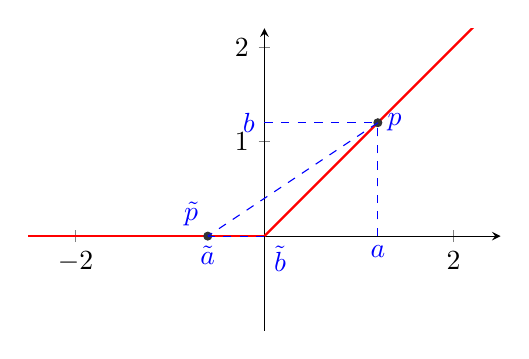
\begin{tikzpicture}
            \begin{axis}[
                axis lines=middle,
                y=1.2cm,
                x=1.2cm,
                xmax=2.5,
                xmin=-2.5,
                xtick={-2,0, 2},
                ymin=-1,
                ymax=2.2,
                ytick={0,1, 2},
                width=2cm
            ]
        
        
            \addplot [domain=-10:0, samples=100,
                      thick, red] {0};
                
            \addplot [domain=0:10, samples=100,
            thick, red] {x};

            \node at (axis cs:-0.6,0) [circle, scale=0.3, draw=black!80,fill=black!80] {};
            \node at (axis cs:1.2,1.2) [circle, scale=0.3, draw=black!80,fill=black!80] {};

            %\addplot[domain=0:1.2, dashed, color=blue] {1.2};
            \tikzstyle{dashed}=[dash pattern=on 3pt off 3pt,color=blue]
            \draw[dashed] (0,1.2) node[left] {$b$} -- (1.2,1.2) node[right] {$p$};
            \draw[dashed] (1.2,0) node[below] {$a$} -- (1.2,1.2) node[right] {};
            \draw[dashed] (1.2,1.2) node[below] {} -- (-0.6,0) node[right] {};
            \draw[dashed] (0,0) node[below right] {$\Tilde{b}$} -- (-0.6, 0) node[above left] {$\Tilde{p}$};
            \draw[dashed] (-0.6, 0) node[below] {$\Tilde{a}$};
            \addplot[mark=none, dashed, color=blue] coordinates {(1.2, 0) (1.2, 1.2)};
            %\addplot+[sharp plot, color=blue] coordinates {(-0.5,0) (1.2,0) (1.2,1.2) } node[below=0.5mm, pos=-0.01,color=blue] {$x_1$}
    %node[below=15mm,color=blue] {$x_2$}
    %node[above=0.5mm,color=blue] {$y_2$};
        
        \end{axis}
        \end{tikzpicture}
        %\end{scaletikzpicturetowidth}
        \[ \relu(x) = \left\{ \begin{array}{ll}
            x, & \mbox{$x \geq 0$}\\
            0, & \mbox{$x < 0$}\end{array} \right. 
        \]
        \caption{An illustration of the $\relu$ function. $p$ and $\Tilde{p}$ are on the two different branches of $\relu$. The slope between any two points on the function is always within $[0,1]$.}\label{fig:relu}
        %\end{subfigure}
        \end{figure}
%We will point out how we could handle some other activation functions when we specify different reasoning for activation functions.

%%\paragraph{Recurrent structures} TBC
%\paragraph{Neural-network verification}We The problem we aim to address is to estimate the change in the output given an $\ell_p$-perturbations on the input. For verification purposes, we need to upper bound the change. The challenge is to derive a \emph{precise} (small) upper bound \emph{efficiently}. We will present the symbolic reasoning framework to address this problem, under different settings.

\paragraph{Shor's relaxation scheme}
We symbolize the computation components in the network and then constrain them with quadratic relations. The verification tasks are exactly encoded as QPs.
Unfortunately, QPs are generally $\NP$-hard to solve, because quadratic programs are quite expressive, and discrete conditions can be captured by them. For example, the MAXCUT problem can be easily expressed as a QP~\cite{maxcut}. To enable efficient solving, we relax the QP to the SDP that can be solved within polynomial time, using Shor's relaxation scheme~\cite{shor_SDP}. Shor's relaxation comes in two forms, which can be viewed as dual to each other~\cite{modern_co}.

The primal relaxation scheme is to relax each scalar variable to a multidimensional vector, and the dual form can be viewed as the Lagrangian relaxation of the original problem. In this work, we mainly use the primal form, so we provide some introduction here. The full detail of both forms of relaxation can be found in~\cref{sec:shor}.

Consider a general quadratic program:
\begin{align}\label{eq:quad-prog}
\begin{split}
    \min \;\;\;&f_0(x) = x^TA_0x+2b_0^Tx+c_0\\ 
    s.t.\;\;\;\;  & f_i(x) = x^TA_ix+2b_i^Tx+c_i \leq 0,\;\forall i\in[m]
\end{split}
\end{align}

We define a dyadic matrix $X(x) = \begin{pmatrix}
1\\
x
\end{pmatrix}\begin{pmatrix}
1\\
x
\end{pmatrix}^T$.

Then $x^T Ax + 2b^Tx+c = \begin{pmatrix}
1\\
x
\end{pmatrix}^T \begin{pmatrix}
&c \;\; &b^T\\
&b \;\; &A
\end{pmatrix}\begin{pmatrix}
1\\
x
\end{pmatrix} = \inprod{\begin{pmatrix}
&c \;\; &b^T\\
&b \;\; &A
\end{pmatrix},X(x)\Big}_F$.

$X(x)$ is the inner product of two vectors, so it is PSD and moreover a rank-1 matrix. If we drop the rank-1 requirement, we can get an SDP:
\begin{equation}\label{eq:prime-sdp}
    \min_{X}\{\inprod{\bar{A}_0,X}_F: \inprod{\bar{A}_i,X}_F\leq 0, i\in[m]; X\succeq 0; X_{11}=1 \},
\end{equation}
where
\[
\bar{A}_i=\begin{pmatrix}
c_i & \;\;\;\;b_i^T \\
b_i & \;\;\;\;A_i
\end{pmatrix}.
\]
The primal form of Shor's relaxation scheme can be viewed as the natural continuous relaxation for some combinatorial problems. We provide a discussion of this in~\cref{sec:shor}.

Given these components, we are ready to see how we can use the framework to verify the feed-forward DNN. We use the two-layer network as an example, and it is straightforward to extend to multi-layer networks within the framework. Let us consider a two-layer network: $f:\R^m\rightarrow \R$, with one hidden layer of dimension $n$:
\begin{equation}\label{eq:2-network}
   f(x) = v\act(Wx+b)+c, 
\end{equation}

where $W\in \R^{n\times m}$, $b\in \R^{n\times 1}$, $v\in \R^{1\times n}$ and $c\in \R$. Let $w_i$ be the $i$-th row vector of $W$.

Given Shor's relaxation scheme and SDP solvers, verifying neural network properties amounts to formulating the tasks as QPs.




\section{Method}
\label{sec:method}

% \ml{``Inconsistent'' to ``large variation''}

% In this section, we propose our methods based on the observations in Section \ref{sec:motivation}.
In this section, we propose two techniques to further enhance the strong baseline to capture the variation of activation distributions better.
We first introduce spatial re-scaling to adapt the network to pixel-to-pixel variation.
We then propose channel-wise shifting and re-scaling to better capture the channel-to-channel variation.
Meanwhile, as both of the two methods are image-dependent, the image-to-image variation can be captured naturally.
By combining the two methods with our strong baseline, we build our enhanced BNN for SR, named EBSR.

% Because the activation distributions among pixels, channels and images have large variations \red{**are highly inconsistent} in SR networks, we introduce spatial re-scaling to adapt to pixel-wise variations and channel shift and re-scaling to adapt to channel-wise variations. And both of them are image-dependent to adapt to image-wise variations, which means during inference our network re-scales and shifts the distributions of activations flexibly for different input images. Based on these methods, we build an enhanced binary neural network for image super-resolution (EBSR).

% According to [3], the difference of activation magnitudes indicates different scaling factors are needed for each pixel.

\subsection{Spatial Re-scaling}
% It is better to use different scaling factors for different pixels to reduce the quantization error and retain more detailed information for image super-resolution. 

% \ml{In the main method, we do not need to introduce the previous works but can focus on introducing our own method. Channel rescaling in Real-to-binary Net is not relevant in this context.}

% Re-scaling the output of binary convolutions was proposed at the birth of BNN in XNOR-Net \cite{rastegari2016xnor} to reduce quantization error and improve accuracy for image classification tasks.
% It is computed as below:
% \begin{equation}
% \mathcal{A} * \mathcal{W} \approx(\operatorname{sign}(\mathcal{A}) \circledast \operatorname{sign}(\mathcal{W})) \odot \mathcal{K} \alpha
% \label{eq:xnor-net rescale}
% \end{equation}
% where $\circledast$ denotes the binary convolution and $\odot$ denotes the element-wise multiplication.
% $\mathcal{A}$, $\mathcal{W}$, $\alpha$, and $\mathcal{K}$ denote the activation, weight, weight scaling factor, and activation scaling factor, respectively.
%  Later in XNOR-Net++ \cite{bulat2019xnor}, Bulat et al. fuse the activation and weight scaling factors into a single one that is learned end-to-end based on gradients and this improves the classification accuracy on ImageNet dataset.

% % It is computed as Eq.~\ref{eq:xnor-net rescale}, where $\circledast$ denotes 
% %  the binary convolution and $\odot$ denotes the element-wise multiplication. The binary convolution of $\mathcal{A}$ and $\mathcal{W}$ is rescaled by the weight scaling factor $\alpha$ and the activation scaling factor $\mathcal{K}$, both of which are calculated analytically.


% \zc{Similarly, you should explain the meaning of A, W and the operators $\circledast$ in the formula}
% Then in Real-to-binary Net \cite{martinez2020training}, Martinez et al. used a data-driven channel re-scaling module that takes the pre-convolution activations as input to predict the activation scaling factor. Unlike that in XNOR-Net++ \cite{bulat2019xnor}, these scaling factors are not fixed during inference but rather inferred from data. By doing this, they further improved the classification accuracy on ImageNet over XNOR-Net++. 
As is shown in Figure \ref{fig:pixel}, activation distributions have large pixel-to-pixel variation in SR networks
and the difference of activation magnitudes indicates different scaling factors are preferred for different pixels.
Inspired by \cite{martinez2020training}, we propose spatial re-scaling to better adapt the network to the spatial variation
of activation distributions in SR networks.
% fit the various pixel-wise distributions in SR networks.
We take the real-valued activations $A$ before convolution as input and predict pixel-wise scaling factors $S(A)$, which re-scale the binary convolution output. Spatial re-scaling process can be formulated as follows:
\begin{equation}
A * W \approx(\operatorname{sign}(A) \circledast \operatorname{sign}(W)) \odot \alpha \odot S(A)
\label{eq:spatial rescale}
\end{equation}
where $\circledast$ denotes 
the binary convolution and $\odot$ denotes the element-wise multiplication. $A$, $W$, $\alpha$, and $S\left(A\right)$ denote real-valued activations, weights, the scaling factor of weights, and the spatial-wise scaling factor of activations respectively. $S\left(A\right) \in \mathbb{R}^{1\times H\times W}$ can be calculated with a convolution and a sigmoid function.
% as $\sigma\left( CONV\left(A\right)\right)$. 
As shown in Figure \ref{fig:method}(a), real-valued activations first go through a convolution layer,
which has an input channel of $C$ and an output channel of 1, 
and then pass through a sigmoid function to produce the scaling factors $S(A)$ along the spatial dimension.
During inference, the scaling factor will change dynamically according to different input feature maps.
By re-scaling binary convolution output using $S(A)$, we can reduce the quantization error and the original pixel-wise information in FP activation
will be preserved much better.
Spatial re-scaling leads to a large PSNR improvement of 0.24 dB (from 30.30 dB to 31.54 dB) on Set5 and 0.22 dB (from 25.09 dB to 25.31 dB)
on Urban100 compared with our strong baseline. 

\subsection{Channel-wise Shifting and Re-scaling}

\begin{table}[!tb]
\centering
\caption{Comparison between whether to fuse channel-wise shifting and re-scaling or not based on our baseline with spatial re-scaling. }
\label{tab:fusing}

\scalebox{0.65}{
\begin{tabular}{c|cc|cc|cc}
\hline
\multirow{2}{*}{Method}     & \multirow{2}{*}{OPs} & \multirow{2}{*}{Params} & \multicolumn{2}{c|}{Set5} & \multicolumn{2}{c}{Urban100} \\ \cline{4-7} 
                            &                      &                         & PSNR        & SSIM        & PSNR          & SSIM         \\ \hline
Baseline + spatial re-scale & 2.16G                & 0.05M                   & 31.54       & 0.883       & 25.31         & 0.759        \\
+ channel-wise shift and re-scale             & 2.34G                & 0.09M                   & 31.61       & 0.885       & 25.35         & 0.761        \\
+ w/ fusing                   & 2.27G                & 0.08M                   & \textbf{31.64}       & \textbf{0.885}       & \textbf{25.36}         & \textbf{0.761}        \\ \hline
\end{tabular}
}
\end{table}

In SR networks, activation distributions exhibit larger channel-to-channel variation (Figure \ref{fig:chl}).
Both the mean and magnitude of the activation distributions vary significantly across channels.
% Thus we use channel-wise shifting and re-scaling to adapt to various channel-wise distributions. 
\cite{martinez2020training} has proposed the data-driven channel re-scaling, 
but our method differs from them in further introducing data-driven thresholds to handle the channel-wise variation of both mean and magnitude.
Since the blocks to generate the scaling factors and thresholds are very similar, we further propose to fuse them into one module.
% and fusing channel-wise shifting and re-scaling into one module.
We evaluate the effect of fusing the two blocks in Table \ref{tab:fusing}.
With channel-wise shifting and re-scaling fused, our models have fewer operations and parameters overhead and slightly higher performance.

For the specific process, we take the real-valued activations as input and predict different thresholds and scaling factors for each channel. They are also image dependent, e.g., $\beta_{i}$ in Eq.\ref{eq:act_binarize} is no longer fixed during inference but generated according to different input feature maps. Channel-wise shifting and re-scaling can be formulated as follows:
\begin{equation}
A * W \approx(\operatorname{sign}(A-C_s(A)) \circledast \operatorname{sign}(W)) \odot \alpha \odot C_r(A)
\label{eq:channel-wise_shift_and_rescale}
\end{equation}
where $\circledast$ denotes 
the binary convolution and $\odot$ denotes the element-wise multiplication. $C_s(A), C_r(A) \in \mathbb{R}^{C\times1\times1}$ denote the channel-wise threshold and scaling factor, respectively. 
We show the block diagram in Figure \ref{fig:method}(b).
The real-valued input feature map is first squeezed to a ${C\times1\times1}$ vector by a global average pooling (GAP) layer.
The subsequent fully connected layers and ReLU learn the channel-wise information and output a ${2C\times1\times1}$ vector.
Then the ${2C\times1\times1}$ vector is split into two ${C\times1\times1}$ vectors.
We use the first $C$ channels as the channel-wise bias and pass the last $C$ channels through a sigmoid layer 
as the channel-wise scaling factor, which are used to shift the real-valued activations and re-scale the binary convolution output, respectively. 


% \ml{We can mention previously, channel-wise re-scale has been proposed. We propose to fuse them. Add the comparison between fuse v.s. no fuse.}

\begin{figure}[!tbp]%
  \centering
    \includegraphics[width=0.4\textwidth]{fig/methods.png}
  
% \subfloat[channel-wise shifting\&re-scale]{
%     \label{subfig:channel-wise shifting and re-scale}
%     \includegraphics[width=0.2\textwidth]{fig/chl shift and rescale.png}
%   }

  \caption{Block diagram for spatial re-scaling, and channel-wise shifting and re-scaling.} 
  % Input A is the real-valued activation tensor and C, H, and W denote its dimension. GAP stands for global average pooling. The reduction ratio r is set to 16 for a better trade-off between the performance and the number of operations and parameters.}
  \label{fig:method}
\end{figure}


\subsection{Network Structure}

Combining the spatial re-scaling and the channel-wise shifting and re-scaling methods, we construct the enhanced convolution layer (E-Conv).
Then we build our EBSR model based on E-Conv.
In Figure \ref{fig:E-conv}, we compare the binary convolution layer used in the baseline network and our proposed E-Conv.
We use spatial and channel-wise scaling factors to re-scale the binary convolution output,
and use channel-wise shifting to learn appropriate thresholds for each channel before binarization.
The scaling factors and threshold used in E-Conv are learnable and depend on the real-valued input activations.
In this way, our proposed EBSR can adapt to pixel-to-pixel, channel-to-channel, and image-to-image variations
to reduce the large binarization error and preserve more details.
% In this way, our proposed E-Conv reduces the large quantization error caused by binarization and keeps the original information of input feature maps to a large extent.


\begin{figure}[!tb]%
  \centering

    \includegraphics[width=0.5\textwidth]{fig/E-conv.png}

  \caption{Comparison of (a) the binary convolution layer with a skip connection used in our baseline network and (b) the proposed E-Conv.}
  \label{fig:E-conv}
\end{figure}


Figure \ref{fig:network} shows the basic block based on the E-Conv and our EBSR composed of the basic blocks. Following existing works, the convolution layers in the head and tail modules are not binarized. We choose the lightweight EDSR which has 16 basic blocks and 64 channels, and EDSR which has 32 basic blocks and 256 channels as our backbones, which correspond to EBSR-light and EBSR, respectively.

\begin{figure}[!tb]%
  \centering
  {
    \includegraphics[width=0.35\textwidth]{fig/network.png}
  }
  
  \caption{The structure of our proposed EBSR.  Convolution layers in purple are real-valued vanilla 3x3 convolutions.}
  \label{fig:network}
\end{figure}
\section{Power of Symbolic Reasoning}\label{sec:power}
In this section, we examine a few tasks beyond the feed-forward network verification. These tasks appear challenging for non-symbolic domains, but can be naturally solved with our framework. We can assign any computational component in the network with a symbol on demand without defining the abstract interpreter a priori. This flexibility contributes to the power of symbolic reasoning.

The major distinguished components of our framework are the symbolic domain and the quadratic relation. The symbolic domain has very flexible semantics. We can assign symbols to any computation component in the network, and define their semantics as needed. In the meantime, the quadratic relation is quite expressive, allowing us to exactly encode the verification problem of interest. We can then use algebraic manipulations and other mathematical tools to precisely analyze those problems. Moreover, using quadratic relations to exactly express the verification problem enables us to ask important theoretical questions about the verification task, which we will discuss in~\cref{sec:theory}. Now we demonstrate the practical benefits with the following examples.

\subsection{Metric Learning}
Metric learning models learn a metric that captures the semantic features. They map inputs into a low-dimensional space on which distance measures the similarity. This model is widely used in face recognition, information retrieval and phishing detection~\cite{phishNet,facenet,Wu_2017_ICCV}. The model structure is essentially the same as the feed-forward except for the final classification layer. Instead of outputting the class with the highest logit score, the model maps the output from the representation layer onto a unit sphere, and outputs the closest anchor's class. 

More formally, let $z$ be the output of the representation layer, and $\bar{z}$ be the normalized $z$, i.e., $\bar{z} = \frac{z}{\norm{z}_2}$. $O = \{o_i\}$ is a set of anchors on the unit sphere (so $\norm{o_i}_2=1$). To predict $x$, the model examines the $\ell_2$-distance between $\bar{z}$ and all the anchors, and outputs the class of the closest anchor.  

\cite{adv-metric} found that metric learning models are also susceptible to adversarial attacks. It appears difficult to verify the metric learning model using non-symbolic domains. Reinterpreting the normalization operation and the $\ell_2$-distance on a unit sphere can be particularly challenging for those domains. However, we demonstrate that with symbolic reasoning, verifying metric learning models is no different from the standard feed-forward model.

Let $o$ be the closest anchor, and $\Tilde{o}$ be another arbitrary anchor. Therefore, we want to minimize $(\bar{z}-\Tilde{o})^2-(\bar{z}-o)^2$ to see if this expression can be negative. With some arithmetical operations:
\[(\bar{z}-\Tilde{o})^2-(\bar{z}-o)^2 = \bar{z}^2+\Tilde{o}^2-\bar{z}^2-o^2+2(o-\Tilde{o})\bar{z}.\]

Because $o^2, \Tilde{o}^2, \bar{z}^2=1$, this is equivalent to minimizing $(o-\Tilde{o})\bar{z}$. Geometrically, this means whether the angle between $\bar{z}$ and $(o-\Tilde{o})$ is greater than $\frac{\pi}{2}$. Therefore, this is equivalent to whether $z$ can be perturbed to the other side of the half-space that is normal to $(o-\Tilde{o})$. 

Equivalently, we only need to minimize $(o-\Tilde{o})z$ to see whether this can be negative. Now assuming the metric learning model has only two layers as in~\cref{eq:2-network}, the quadratic program for metric learning is then:
\begin{align*}
    \min &\;(o-\Tilde{o})z\\ 
    s.t.\;\;\;\;  & z_i(z_i-y_i)\leq 0, \;z_i\geq y_i, \;z_i\geq 0, \;\forall i\in [n] \\
    &y_i = w_i x+b_{1i},\;\forall i\in [n] \\
    &\norm{x-a}_p\leq \epsilon .
\end{align*}

With symbolic reasoning, we can conclude that verifying metric learning models is essentially the same as the standard classification model. We can use a vector $v$ to denote $\Tilde{o}-o$, then the program is the same as in the standard feed-forward model.

\subsection{Deep Equilibrium Models}
Symbolic abstraction is a fundamental reasoning scheme and is used beyond program verification. It can be particularly elegant when reasoning the limiting behavior of recursions. We provide a probability theory example to show this reasoning in~\cref{sec:rec-prob}. We assign the symbol with semantics in the limiting state directly without handling fixed points. Now we demonstrate this reasoning in the verification setting.

We show that we can easily reason about the deep equilibrium (DEQ) model~\cite{deq_model}. DEQs use a single implicit layer to simulate a network with infinite depth. It is based on the observation that very deep models converge towards some fixed point, and the implicit layer solves this fixed point directly. It has been shown that DEQs have competitive performance compared to explicit deep models while consuming much less memory~\cite{multi-deq}.

The DEQ model $f:\R^m\rightarrow \R$ can be described with the following formula:
\[f(x) = vz+b_2, \;z = \act(Wz+Ux+b_1).\]
If we compare the DEQ model with the feed-forward model (see~\cref{eq:2-network}), the difference is that $z$ is also fed back to the input of the hidden layer, i.e., $z$ is a fixed point of the hidden layer equation. The model then uses the affine transformation of this fixed point to make predictions, i.e., $\class(f,x)=\argmax_{i\in[l]}Vz+b$, where $V$ is the weight matrix from the fixed point $z$ to the logit layer, and $b$ is the bias term.

If we assign a non-symbolic domain to capture the semantics of $x$, reasoning $z$ requires finding the fixed point within this domain, which can be very loose. Instead, we can assign symbols to denote the equilibrium behavior directly. We use the FGL estimation (see~\cref{sec:indept}) as an example. 

To derive the QP like~\cref{eq:formal}, the only difference between the DEQ model and the feed-forward DNN is that $\Delta y_i = w_i\Delta z + u_i\Delta z$, where $u_i$ is the $i$-th row of $U$. In other words, an input to the hidden layer ($\Delta y_i$) comes from both the input layer ($w_i\Delta x$) and the output of the hidden layer ($u_i\Delta z$). The rest remains the same. As a result, the QP for the FGL estimation of DEQ is:
\begin{align*}
\begin{split}
  \max &\;v\Delta z \\ 
    s.t.\;\;\;\;  & (\Delta z_i - \Delta y_i)\Delta z_i\leq 0, \;\forall i\in [n] \\
    & \Delta y_i = w_i \Delta x+u_i\Delta z, \;\forall i\in [n]\\
    &\norm{\Delta x}_p\leq 1.
\end{split}  
\end{align*}
%It is easy to see that to certify the robustness of an input for DEQ models, we only need to change~\cref{eq:first-layer} to
%\[
%y_i = w_i x + u_i z+ b_{1i}.
%\]

%\subsection{Transferring $\ell_\infty$-techniques}\label{sec:linf2l2}
%Most of the verification works are focused on the $\ell_\infty$-attacks. One of the reasons is that $\ell_\infty$-attacks are easy to express with linear relations. However, we can adapt some of the techniques designed for $\ell_\infty$-attacks to the $\ell_2$-ones with symbolic reasoning and quadratic relations. 

%For $\ell_\infty$-certification techniques, they often use $l$ and $u$ for each node to denote the lower and upper bounds, and then relate them to over-approximate the NN execution. From symbolic reasoning, we can view $l$ and $u$ as extra symbols, and then quantify them using quadratic relations. This allows us to transfer some of the $\ell_\infty$-techniques to the $\ell_2$-robustness certification. We provide some discussion in~\cref{sec:adapt}.

%For $\ell_infty$ attacks, the verification techniques usually associate two symbols $u$ and $l$ with each node in the network. The semantics of these two variables are each node's upper and lower bounds. Then the NN execution is defined with respect to the lower and upper bounds of each node. As a result, to adapt the $\ell_\infty$-techniques to the $\ell_2$-attacks, we only need to express $\ell_2$-balls with the $u_i$'s and $l_i$'s on the input layer. 

%More formally, suppose we want to express the $\ell_p$-ball centered at $a\in \R^m$ with radius $\epsilon$.

%For $\ell_\infty$-attacks, $u_i$ and $l_i$ can be calculated directly: $u_i=a_i-\epsilon$ and $l_i=a_i-\epsilon$. For $\ell_2$-attacks, if we calculate the concrete values that over-approximate the $\ell_2$-ball, this becomes the $\ell_\infty$-ball and a very loose over-approximation. However, if we view them as symbols rather than concrete values, we can easily express the $\ell_2$-ball and adapt the techniques for $\ell_\infty$-attacks. We provide a more detailed discussion on this in~\cref{sec:adapt}.

\section{Empirical Evaluation}\label{sec:empirical_res} Building on insights
gained from our ablations discussed in Section~\ref{sec:sift_ablations}, we
apply Sparse-IFTs to ImageNet (Section~\ref{subsec:imagenet}), also
demonstrating its advantages for transfer learning in various computer vision
tasks. Additionally, we highlight the benefits of Sparse-IFT in the domain of
NLP by presenting results on GPT~\citep{brown2020language} in
Section~\ref{subsec:nlp_results}.

\begin{table}
    \caption{Sparse Wide IFT with various efficient architectures on CIFAR-100
across different levels of sparsity (columns).} 
    \centering
    \begin{sc}
    \begin{small}
    \resizebox{0.70\linewidth}{!}{
    \begin{tabular}{c|ccc}
        \toprule
        	    & Dense             & 0.50 & 0.75 \\ \midrule MobileNetV2 & 72.4
        $\pm$ 0.2    & 73.4 & \textbf{73.7} \\
        MobileViT-S & 73.5 $\pm$ 0.1    & 74.6 & \textbf{74.8} \\
        BotNet-26   & 78.0 $\pm$ 0.2    & 78.1 & \textbf{78.7} \\
        BotNet-50   & 79.8 $\pm$ 0.2     & 80.3 & \textbf{80.9} \\
        \bottomrule
    \end{tabular}
    }
    \end{small}
    \end{sc}
\label{tab:mbv2-cifar}
\end{table}

\begin{table}
        \caption{Sparse-IFT on ImageNet. Best result for each transformation and
    architecture is highlighted in bold.}
        \begin{center}
        \begin{small}
        \begin{sc}
        \resizebox{\linewidth}{!}{
        \begin{tabular}{c|c|c|ccc}
            \toprule
            Model & Dense & Transformation & 0.50 & 0.75 & 0.90 \\
    \midrule
            \multirow{2}{*}{ResNet-18} &  \multirow{2}{*}{70.9 $\pm$ 0.1} &
    Sparse Wide & 72.7 & 73.8 & \textbf{74.4} \\
            &   & Sparse Parallel & 72.7 & 73.2 & \textbf{74.0} \\ \midrule
            ResNet-34 & 74.2 $\pm$ 0.1 & Sparse Wide &  75.6 & 76.4 &
            \textbf{76.8} \\ \midrule BotNet-50 & 77.5 $\pm$ 0.1 &  Sparse Wide
            & 77.9 & 78.3 & \textbf{78.5} \\
            \bottomrule
        \end{tabular}
        }
        \end{sc}
        \end{small}
    \end{center}
    \label{tab:resnet-i1k}
\end{table}

\subsection{ImageNet}
\label{subsec:imagenet}
We apply the best-performing Sparse-IFT transformations (Sparse Wide IFT and
Sparse Parallel IFT) from CIFAR-100 to ImageNet using ResNet-18. We follow
published training settings for ImageNet~\citep{nvidia2023gpuperf}. Both
Sparse-IFT families achieve significantly higher accuracy compared to the dense
baseline (see Table~\ref{tab:resnet-i1k}). Specifically, Sparse Wide IFT
ResNet-18 at 90\% sparsity improves over the dense baseline by 3.5\% and matches
the accuracy of a dense ResNet-34 with 2× fewer training FLOPs (refer to
Figure~\ref{fig:sift_resnet_improvement}). We also apply the best-performing
transformation (Sparse Wide IFT) to ResNet-34 and BotNet-50. Increasing sparsity
consistently improves accuracy, indicating enhanced training efficiency at
higher sparsities. On BotNet-50, a hybrid ViT model, there is a 1.1\%
improvement at 90\% sparsity.

\subsection{Transfer Learning on Downstream Tasks}
\label{subsec:transfer_learning}
To show the effectiveness of pre-training our Sparse-IFT classification
backbones, we evaluate them on 1) object detection on MS COCO
2017~\cite{lin2014microsoft}, and 2) semantic segmentation on
CityScapes~\cite{cordts2016cityscapes}. For object detection, we adopt
RetinaNet~\cite{lin2017focal} from the MMDetection open-source
toolbox~\cite{mmdetection} and report results in the standardized training
setting. For semantic segmentation, we utilize DeepLabV3+~\cite{chen2018encoder}
in the MMSegmenation open-source toolbox~\cite{mmseg2020}. We evaluate ResNet-18
with Sparse Wide IFT and to ensure FLOP-equivalent comparisons with the dense
backbone, the Sparse-IFT backbones remain sparse during fine-tuning.
Appendix~\ref{app:eval_downstream} provides more details on the training setup.
We summarize our findings in Table \ref{tab:down_stream}, where using Sparse
Wide IFT ResNet-18 backbone leads to significant accuracy gains across all
metrics on both tasks.

\begin{table}
    \caption{Sparse Wide IFT variants of ResNet-18 as backbones for: (a) object
detection on MS COCO, (b) semantic segmentation on Cityscapes.} 
    \centering
    \begin{small}
    \begin{sc}
    \resizebox{0.8\linewidth}{!}{
    \begin{tabular}{c|c|cccc}
        \toprule
      & Metric & Dense & 0.50   & 0.75  & 0.90 \\
    \midrule
 \multirow{3}{*}{MS COCO}     &  AP      &  29.3  & 31.3 & 32.8 & \textbf{34.5}
 \\
      &  AP$_{50}$    &  46.2  & 49.0 & 51.0 & \textbf{53.5} \\
      &  AP$_{75}$    &  30.9  & 33.0 & 34.8 & \textbf{36.5} \\
    \midrule
  \multirow{2}{*}{CityScapes}     &  \text{mIoU}      &   76.7   &  77.9   &
  78.9 & \textbf{79.1} \\
      &  \text{mAcc}      &   84.4   &  85.1   & 85.7 & \textbf{86.0} \\
        \bottomrule
    \end{tabular}
    }
    \end{sc}
    \end{small}
\label{tab:down_stream}
\end{table}

\begin{table}
    \caption{Average accuracy of Sparse Wide IFT with GPT-3 Small across ARC,
     HellaSwag, TruthfulQA, MMLU and Winogrande tasks on the Open LLM
     Leaderboard.} 
    \begin{center}
    \begin{small} 
    \begin{sc}
    \resizebox{0.7\linewidth}{!}{
    \begin{tabular}{cc|cc}
        \toprule
       	Model	     & Dense & 0.50 & 0.75 \\

	\midrule
        GPT-3 Small &   33.8 $\pm$ 0.1  &  34.1      &  \textbf{34.7}  \\
        \bottomrule
    \end{tabular}
    }
    \end{sc}
    \end{small}
    \end{center}
\label{tab:nlp_scratch_result}
\end{table}

\subsection{Language Modeling}
\label{subsec:nlp_results} 
We pre-train the Sparse Wide IFT GPT-3 Small model at $s \in \{50\%, 75\%\}$
from scratch on the Pile~\citep{gao2020pile} dataset using the
SET~\citep{mocanu2018}, and compare against the standard dense model. All models
were trained on the Cerebras CS-2~\citep{lie_2023} following
Chinchilla~\citep{hoffmann2022an} for obtaining loss-optimal pre-trained
baseline configurations of models. We evaluate the models on 5 tasks from the
Open LLM leaderboard~\citep{open-llm-leaderboard} (i.e.,
ARC~\citep{clark2018think}, HellaSwag~\citep{zellers2019hellaswag},
MMLU~\citep{hendrycks2021measuring}, TruthfulQA~\citep{lin2022truthfulqa} and
Winogrande~\citep{DBLP:journals/corr/abs-1907-10641}), and show that the Sparse
Wide IFT GPT-3 Small at 75\% sparsity improves the average accuracy by a
noticeable 0.9\% (see Table~\ref{tab:nlp_scratch_result}). In
Appendix~\ref{app:gpt_e2e}, we provide details on the models and
hyperparameters.
We provide some comments on the growth conditions which constituted the majority of our analysis in sections \ref{sec:Hmixing} and \ref{sec:Hsigma}. In the simplest cases of Lemma \ref{lemma:unstableGrowth}, growth was established in an analogous fashion to the old one-step expansion condition (\ref{eq:oldOneStepExpansion}), finding the relevant Jacobians $M_j$ and checking that their expansion factors $K(M_j)$ satisfy
\begin{equation}
    \label{eq:discussionOneStep}
    \sum_j \frac{1}{K(M_j)} <1.
\end{equation}
For the more complicated cases, the inductive method used to establish growth near the accumulation points in Lemma \ref{lemma:unstableGrowth} and the weakened one-step expansion condition (\ref{eq:oneStep}) both address the same fundamental issue: the splitting of unstable curves by singularities into an unbounded number of small components. They circumvent this obstacle in rather different ways, however. While (\ref{eq:oneStep}) generalises (\ref{eq:discussionOneStep}) to ensure an growth of unstable curves `on average' (see \cite{chernov_statistical_2009} for a precise statement), our inductive method is a more direct adaptation of (\ref{eq:discussionOneStep}), using it to generate contradictory geometric conditions which a hypothetical non-growing unstable curve must satisfy. It may be possible to prove Theorem \ref{sec:Hmixing} using (\ref{eq:oneStep}) as the basis for growth. Since we required (\ref{eq:oneStep}) anyway for proving Theorem \ref{thm:HsigmaExp}, this could potentially condense our analysis, but only to a minor extent. A convenience of the method used in section \ref{sec:Hmixing} is that, by way of the `simple intersection' property, it naturally gives geometric information on the images of manifolds, useful for proving the property \textbf{(M)} of Theorem \ref{thm:katok-strelcyn}.

We expect that essentially analogous analysis can be applied to establish mixing properties in a wide class of piecewise linear non-uniformly hyperbolic maps, including those (like the OTM) which sit on the boundary of ergodicity and beyond. While we have relied on the precise partition structure of $H_\sigma$, its fundamental feature (self-similar sequences of elements $A^k$, sharing boundaries with its neighbours $A^{k-1},A^{k+1}$ and accumulating onto some point $p$) is quite typical to return map systems. See, for example, those of various stadium billiards \cite{chernov_chaotic_2006,chernov_improved_2008,chernov_statistical_2009} and LTMs \cite{springham_polynomial_2014}. Indeed, the same method can be used to prove the Bernoulli property for non-monotonic LTMs \cite{myers_hill_mixing_2022}, where monotonicity of the manifold images cannot be assumed and the classical argument \cite{sturman_mathematical_2006} fails. The OTM is the pointwise limit of these maps as the boundary shrinks to null measure. It further has utility in proving growth conditions for maps which are uniformly hyperbolic but possess regions $A_j$ where the hyperbolicity is very weak, signified by $K(M_j) \approx 1$, so that (\ref{eq:discussionOneStep}) fails. Typically this leads to suboptimal bounds on mixing windows, see e.g. \cite{wojtkowski_model_1981,przytycki_ergodicity_1983,myers_hill_family_2022}. The map $H_{(\eta,\eta)}$ for $\eta \approx 1/2$ is another example, possessing weak hyperbolicity over $A_2, A_3$. Letting $\varepsilon = |\eta-1/2|>0$, there is an upper bound $N = N(\varepsilon)$ on escape times from the intersections $A_2\cap \sigma, A_3 \cap \sigma$. The growth lemma then follows by applying the inductive step roughly $N$ times and can be established for arbitrarily small $\varepsilon$, opening the door to establishing optimal mixing windows.

The above gives two examples of piecewise linear perturbations to $H$ where mixing with respect to Lebesgue is preserved and our methods can be applied. Nonlinear perturbations to the shear profiles complicate the analysis in several ways. Firstly as the map's Jacobians takes on a broader range of values, cone invariance becomes an increasingly harder condition to establish. Cones must be widened, giving looser bounds on expansion factors, which may already be weak due to new regions of weaker stretching. This, together with the change from polygonal to curvilinear return time partition elements and nonlinear local manifolds, adds some complexity to showing growth conditions. This does not rule out certain (small) nonlinear perturbations however. There is some leeway in the inequalities which govern cone invariance and growth of local manifolds, the latter of which is not too dissimilar from the piecewise linear setting (see Lemmas \ref{lemma:piecewiseApprox}, \ref{lemma:componentLength}). Certain small perturbations would not alter the \emph{topological} structure of the return time partition, i.e. which elements share boundaries, the key information needed for setting up the induction. Finally while the partition elements would no longer be polygonal, only coarse geometric information is required for verifying each inductive step. Following the above, a potential perturbation could be to replace the linear portions of each shear by a cubic, perturbing the tent profile
\[  f(t) = \begin{cases} 2t & 0 \leq t \leq 1/2, \\ 2(1-t) & 1/2 \leq t \leq 1 ,\end{cases} \]
of the OTM shears to
\[  f_a(t) = \begin{cases} \frac{1}{8} t \left(16 - a + 6at - 8at^{2} \right) & 0 \leq t \leq 1/2, \\ \frac{1}{8}\left(1-t\right)\left( 16 - a + 6a\left(1-t\right) - 8a\left(1-t\right)^{2}\right)  & 1/2 \leq t \leq 1, \end{cases}   \]
for $a>0$. For small enough $a$ the gradient range $f'(t)$ is restricted to small neighbourhoods of $\{ 2, -2\}$ and the escape time partition retains a similar structure. We illustrate this in Figure \ref{fig:perturbations}, showing escapes from the square $S_3$ under the map $G \circ F$, equivalent to escapes from the perturbed $A_3$ under the $G \circ F$, but with a cleaner geometry for comparison. When $a$ is too large the analogy to the OTM breaks down. At $a=16$ the map is twice differentiable everywhere and features a new source of slowed mixing, the Jacobian is the identity at the corner points $x,y \in \{  0, 1/2 \}$ giving locally parabolic behaviour (visible in the escape time partition). 

\begin{figure}
    \centering
    \includegraphics[width=0.24 \linewidth]{0.png}
    \includegraphics[width=0.24 \linewidth]{4.png}
    \includegraphics[width=0.24 \linewidth]{8.png}
    \includegraphics[width=0.24 \linewidth]{16.png}
    \caption{Partition of escape times from $S_3$ under the mapping $F \circ G$ for $a= 0,4,8,16$. }
    \label{fig:perturbations}
\end{figure}
\section{Related work}
\noindent \textbf{Video foundation models.}
With sufficient computational power and an abundant source of data, there have been attempts to build a single large-scale foundation model that can be adapted to diverse downstream tasks.
Along with the success of foundations models in the natural language processing domain~\cite{brown2020language,chen2021evaluating,devlin2019bert} and in computer vision~\cite{bertasius2021space,jia2021scaling,radford2021learning}, video data has become another data type of interest, as it has grown in scale due to numerous internet video-sharing platforms.
Accordingly, several methods to train a video foundation model have been proposed.
Due to the innate multi-modality of video data, \textit{i.e.}, a combination of visual $\cdot$ vocal $\cdot$ textual context, most works have centered around the variations of the cross-modal attention mechanism \cite{akbari2021vatt,bertasius2021space,gabeur2020multi,luo2020univl,neimark2021video,tan2021look,wei2020multi,yang2021taco}.
In addition, as most video data lack proper labels or descriptions, contrastive learning methods were studied to learn meaningful feature representations or enhance video-text alignment in a self-supervised manner \cite{akbari2021vatt,kuang2021video,luo2020univl,yang2021taco}.

More specifically, MERLOT \cite{zellers2021merlot} proposed a multi-modal representation learning method for visual commonsense reasoning, which also performed well in twelve video reasoning tasks.
VATT \cite{akbari2021vatt} introduced a multi-modal learning method via contrastive learning. 
The pre-trained model performed well in a variety of vision tasks from image classification to video action recognition and zero-shot video retrieval.
Another representative work, UniVL \cite{luo2020univl} proposed a straightforward pre-training method with auxiliary loss functions. 
After fine-tuning on a specific task, the pre-trained model performed outstandingly in a wide range of tasks of text-to-video retrieval, action segmentation, action step localization, video sentiment analysis, and video captioning.
Other foundation models for multiple video tasks include \cite{li2020hero,sun2019learning,sun2019videobert,zhu2020actbert,fu2021violet,wang2022all}. 

\noindent \textbf{Auxiliary learning.}
In order to enhance the performance of one or a multitude of primary tasks, auxiliary learning methods can be incorporated.
\cite{ruder2017overview} introduced Multi-task learning (MTL) to the deep neural networks by training a single model with multiple task losses to assist learning on the main task.
Such a method is generally adapted to pre-train the foundation models in the self-supervised manner~\cite{li2020hero,sun2019learning,sun2019videobert,zhu2020actbert,fu2021violet,wang2022all}.
However, these various pretext task losses used in the pre-training phase are ignored in the fine-tuning phase, and only the primary task loss is minimized.

Recently, meta-learning methods have been introduced for auxiliary learning.
\cite{liu2019self,navon2020auxiliary,shu2019meta} proposed a meta-learning method in which the model learns auxiliary tasks to generalize well to unseen data. 
In these settings, a separate subset of data is held out as the primary task, while the others are used as auxiliary tasks that aid the primary task's performance.
Similar methods were adopted for computer vision tasks such as semantic segmentation \cite{xu2021leveraging}.
Other domain applications include navigation tasks with reinforcement learning \cite{ye2021auxiliary}, or self-supervised learning methods on graph data \cite{hwang2020self}.
%
% ---- Bibliography ----
%
% BibTeX users should specify bibliography style 'splncs04'.
% References will then be sorted and formatted in the correct style.
%
\bibliographystyle{splncs04}
\bibliography{paper}

\appendix
\section{Appendix for Proofs}

\paragraph{Proof of Theorem \ref{thm:main}.}

\begin{proof}
\label{proof:main}
Our proof has two steps. In Step 1, we will show that SimCLR is equivalent to minimizing the cross entropy loss defined in Eqn.~(\ref{eqn:cross-entropy}). 
In Step 2, we will show  that minimizing the cross-entropy loss 
is equivalent to spectral clustering on $\bfpi$. 
Combining the two steps together, we have proved our theorem. 

\textbf{Step 1: } SimCLR is equivalent to minimizing the cross entropy loss.

The cross-entropy loss takes expectation over 
$\bfW_\bfX\sim \mathbb{P}(\cdot ; \bfpi)$, 
which means $\bfW_\bfX$ has exactly one non-zero entry in each row $i$. By Lemma~\ref{lem:multinomial}, we know every row $i$ of $\bfW_\bfX$ is independent of other rows. Moreover, 
$\bfW_{\bfX,i}\sim \mathcal{M}(1, \bfpi_i/\sum_j \bfpi_{i,j})=\mathcal{M}(1, \bfpi_i)$, because $\bfpi_i$ itself is a probability distribution.
Similarly, we know $\bfW_\bfZ$ also has the row-independent property by sampling over $\mathbb{P}(\cdot;\bfK_\bfZ)$.
Therefore, by Lemma~\ref{lem:cross_split}, we know Eqn.~(\ref{eqn:cross-entropy}) is equivalent to:
\[
 -\sum_{i=1}^n \mathbb{E}_{\bfW_{\bfX,i}}[\log \mathbb{P}(\bfW_{\bfZ,i}=\bfW_{\bfX,i};\bfK_\bfZ)],
\]

This expression takes expectation over $\bfW_{\bfX,i}$ for the given row $i$. Notice that 
$\bfW_{\bfX,i}$ has exactly one non-zero entry, which equals $1$ (same for $\bfW_{\bfZ,i}$). 
As a result
we expand the above expression to be:
\begin{equation}
 -\sum_{i=1}^n \sum_{j\neq i} \Pr(\bfW_{\bfX,i,j}=1)\log \Pr(\bfW_{\bfZ,i,j}=1).
\label{eqn:detailed-expansion}    
\end{equation}


By Lemma~\ref{lem:multinomial}, $\Pr(\bfW_{\bfZ,i,j}=1)=\bfK_{\bfZ,i,j}/\|\bfK_{\bfZ,i}\|_1$ for $j\neq i$. Recall that $\bfK_\bfZ=(k(\bfZ_i-\bfZ_j))_{(i,j)\in[n]^2}$, which means 
$\bfK_{\bfZ,i,j}/\|\bfK_{\bfZ,i}\|_1=\frac{\exp(-\|\bfZ_i-\bfZ_j\|^2/{2\tau})}{\sum_{k\neq i}
\exp(-\|\bfZ_i-\bfZ_k\|^2/{2\tau})
}$ for $j\neq i$, when $k$ is the Gaussian kernel with variance $\tau$. 

Notice that $\bfZ_i=f(\bfX_i)$, so we know
\begin{equation}
-\log \Pr(\bfW_{\bfZ,i,j}=1)=
-\log \frac{\exp(-\|f(\bfX_i)-f(\bfX_j)\|^2/{2\tau})}{\sum_{k\neq i}
\exp(-\|f(\bfX_i)-f(\bfX_k)\|^2/{2\tau}),
}
\label{eqn:infonce-equivalence}    
\end{equation}


The right hand side is exactly the InfoNCE loss defined in Eqn.~(\ref{eqn:infonce}).
Inserting Eqn.~(\ref{eqn:infonce-equivalence}) into Eqn.~(\ref{eqn:detailed-expansion}), we get the SimCLR algorithm, which first samples augmentation pairs $(i,j)$ with $\Pr(\bfW_{\bfX,i,j}=1)$ for each row $i$, and then optimize the InfoNCE loss. 

\textbf{Step 2: } minimizing the cross entropy loss 
is equivalent to spectral clustering on $\bfpi$.


By Lemma~\ref{lem:convert_to_spectral}, we may further convert the loss to 
\begin{equation}
\label{eqn:main-theorem-repul-attr}
\min_{\bfZ}
-\sum_{(i,j)\in [n]^2} \mathbf{P}_{i,j}
\log k (\bfZ_i-\bfZ_j)+\log \mathbf{R}(\bfZ).
\end{equation}
Since $k$ is the Gaussian kernel, this reduces to \[
\min_\bfZ \mathrm{tr}(\bfZ^\top \mathbf{L}(\bfpi) \bfZ)
+\log \mathbf{R}(\bfZ),
\]

where we use the fact that $\mathbb{E}_{\bfW_\bfX\sim \mathbb{P}(\cdot; \bfpi)}[\mathbf{L}(\bfW_\bfX)]
=\mathbf{L}(\bfpi)
$, because the Laplacian operator is linear and $
\mathbb{E}_{\bfW_\bfX\sim \mathbb{P}(\cdot; \bfpi)}(\bfW_\bfX)=\bfpi
$.
\end{proof}

\paragraph{Proof of Theorem \ref{thm:clip}.}
\begin{proof}
Since $\bfW_\bfX\sim \mathbb{P}(\cdot;\bfpi_{\mathbf{A}, \mathbf{B}})$, we know 
$\bfW_\bfX$ has exactly one non-zero entry in each row, denoting the pair that got sampled. 
A notable difference compared to the previous proof is we now have $n_\mathcal{A}+n_\mathcal{B}$ objects in our graph. CLIP deals with this by taking a mini-batch of size $2N$, 
such that $n_\mathcal{A}=n_\mathcal{B}=N$, and adding the $2N$ InfoNCE losses together. We label the objects in $\mathcal{A}$ as $[n_\mathcal{A}]$, and the objects in $\mathcal{B}$ as $\{n_\mathcal{A}+1, \cdots, n_\mathcal{A}+n_\mathcal{B}\}$. 

Notice that $\bfpi_{\mathbf{A}, \mathbf{B}}$ is a bipartite graph, so the edges of objects in $\mathcal{A}$ will only connect to object in $\mathcal{B}$ and vice versa. We can define the similarity matrix in $\cZ$ as $\bfK_\bfZ$, 
where $\bfK_\bfZ(i, j+n_\mathcal{A})=\bfK_\bfZ(j+n_\mathcal{A},i)= k(\bfZ_i-\bfZ_j)$ for $i\in [n_\mathcal{A}], j\in [n_\mathcal{B}]$, and otherwise we set $\bfK_\bfZ(i,j)=0$. 
The rest is same as the previous proof. 
\end{proof}

\paragraph{Proof of Theorem \ref{thm:exponential}.}

\begin{proof}
\label{proof:exponential}
Since the objective function consists of a linear term combined with an entropy regularization, which is a strongly concave function, the maximization problem is a convex optimization problem. Owing to the implicit constraints provided by the entropy function, the problem is equivalent to having only the equality constraint. We then introduce the Lagrangian multiplier $\lambda$ and obtain the following relaxed problem:

$$
\widetilde{E}(\boldsymbol{\alpha})=\psi_{1}-\sum_{i=1}^n \alpha_{i} \psi_{i}+\tau \sum_{i=1}^n \alpha_{i}\log \alpha_{i}+\lambda\left(\boldsymbol{\alpha}^{\top} \mathbf{1}_n-1\right).
$$

As the relaxed problem is unconstrained, taking the derivative with respect to $\alpha_{i}$ yields

$$
\frac{\partial \widetilde{E}(\boldsymbol{\alpha})}{\partial \alpha_{i}}=-\psi_{i}+\tau\left(\log \alpha_{i}+\alpha_{i} \frac{1}{\alpha_{i}}\right)+\lambda=0.
$$

Solving the above equation implies that $\alpha_{i}$ takes the form
$
\alpha_{i}=\exp \left(\frac{1}{\tau} \psi_{i}\right) \exp \left(\frac{-\lambda}{\tau}-1\right).
$ Since $\alpha_{i}$ lies on the probability simplex, the optimal $\alpha_{i}$ is explicitly given by
$
\alpha^{*}_{i}=\frac{\exp \left(\frac{1}{\tau} \psi_{i}\right)}{\sum_{i^{\prime}=1}^n \exp \left(\frac{1}{\tau} \psi_{i^{\prime}}\right)} .
$ Substituting the optimal point into the objective function, we obtain
$$
\begin{aligned}
E\left(\boldsymbol{\alpha}^*\right)  &=\psi_1-\sum_{i=1}^n \frac{\exp \left(\frac{1}{\tau} \psi_{i}\right)}{\sum_{i^{\prime}=1}^n \exp \left(\frac{1}{\tau} \psi_{i^{\prime}}\right)} \psi_{i}+\tau \sum_{i=1}^n \frac{\exp \left(\frac{1}{\tau} \psi_{i}\right)}{\sum_{i^{\prime}=1}^n \exp \left(\frac{1}{\tau} \psi_{i^{\prime}}\right)}\log \frac{\exp \left(\frac{1}{\tau} \psi_{i}\right)}{\sum_{i^{\prime}=1}^n \exp \left(\frac{1}{\tau} \psi_{i^{\prime}}\right)} \\
& =\psi_1 - \tau \log \left(\sum_{i=1}^n \exp \left(\frac{1}{\tau} \psi_{i}\right)\right).
\end{aligned}
$$
Thus, the Lagrangian dual function is given by
\begin{equation*}
-E\left(\boldsymbol{\alpha}^*\right)= -\tau \log \frac{\exp \left(\frac{1}{\tau} \psi_{1}\right)}{\sum_{i=1}^n \exp \left(\frac{1}{\tau} \psi_{i}\right)}.\qedhere
\end{equation*}
\end{proof}



\section{More on Experiments} \label{section: experiment_details}

\paragraph{CIFAR-10 and CIFAR-100} CIFAR-10 ~\citep{krizhevsky2009learning} and CIFAR-100 ~\citep{krizhevsky2009learning} are well-known classic image classification datasets. Both CIFAR-10 and CIFAR-100 contain a total of 60k $32 \times 32$ labeled images of different classes, with 50k for training and 10k for testing. CIFAR-10 is similar to CIFAR-100, except there are 10 different classes in CIFAR-10 and 100 classes in CIFAR-100.

\paragraph{TinyImageNet} TinyImageNet ~\citep{le2015tiny} is a subset of ImageNet ~\citep{deng2009imagenet}. There are 200 different object classes in TinyImageNet, with 500 training images, 50 validation images, and 50 test images for each class. All the images in TinyImageNet are colored and labeled with a size of $64 \times 64$.

\textbf{Pseudo-code.} Algorithm \ref{alg:Training Procedure} presents the pseudo-code for our empirical training procedure.

\begin{algorithm}[!htbp]
\caption{Training Procedure}
\label{alg:Training Procedure}
\begin{algorithmic}[1]
\REQUIRE trainable encoder network $f$, batch size $N$, augmentation strategy \textit{aug}, loss function $L$ with hyperparameters \textit{args}
\FOR {sampled minibatch ${x_i}_{i=1}^N$}
\FORALL{$i \in { 1, ..., N }$}
\STATE draw two augmentations $t_i = \textit{aug}\left(x_i\right) $, $t_i' = \textit{aug}\left(x_i\right) $
\STATE $z_i = f\left(t_i\right)$, $z_i' = f\left(t_i'\right)$
\ENDFOR
\STATE compute loss $\mathcal{L} = L(N, z, z', \textit{args})$
\STATE update encoder network $f$ to minimize $\mathcal{L}$
\ENDFOR
\STATE \textbf{Return} encoder network $f$
\end{algorithmic}
\end{algorithm}

We also provide the pseudo-code for our core loss function used in the training procedure in Algorithm \ref{alg:Core loss}. The pseudo-code is almost identical to SimCLR's loss function, with the exception of an extra parameter $\gamma$.

\begin{algorithm}[!htbp]
\caption{Core loss function $\mathcal{C}$}
\label{alg:Core loss}
\begin{algorithmic}[1]
\REQUIRE batch size $N$, two encoded minibatches $z_1, z_2$, $\gamma$, temperature $\tau$
\STATE $z = \textit{concat}\left(z_1, z_2\right)$
\FOR {$i \in {1, ..., 2N }, j \in {1, ..., 2N}$ }
\STATE $s_{i,j} = \Vert z_i - z_j \Vert_2^{\gamma}$
\ENDFOR
\STATE \textbf{define} $l(i, j)$ \textbf{as} $l(i, j) = - \log \frac{exp\left(s_{i,j}/\tau \right)}{\sum_{k=1}^{2N} \mathbf{1}{[k \ne i]} exp\left(s{i, j} / \tau \right)} $
\STATE \textbf{Return} $\frac{1}{2N} \sum_{k=1}^N\left[l(i, i+N) + l(i+N, i)\right]$
\end{algorithmic}
\end{algorithm}

Utilizing the core loss function $\mathcal{C}$, we can define all kernel loss functions used in our experiments in Table \ref{table: loss definition}. For all $z_i \in z$ with even dimensions $n$, we define $z_{L_i} = z_i\left[0:n/2\right]$ and $z_{R_i} = z_i\left[n/2:n\right]$.

\begin{table}[ht]
\centering
\begin{tabular}{{@{}l|l@{}}}
Kernel  &  Loss function \\ \midrule
Laplacian & $\mathcal{C}\left(N, z, z', \gamma=1, \tau\right)$\\ \midrule
Sum       & $\lambda * \mathcal{C}\left(N, z, z', \gamma=1, \tau_1\right) + (1-\lambda) * \mathcal{C}\left(N, z, z', \gamma=2, \tau_2\right)$  \\ \midrule
Concatenation Sum&$\lambda * \mathcal{C}\left(N, z_L, z'_L, \gamma=1, \tau_1\right) + (1-\lambda) * \mathcal{C}\left(N, z_R, z'_R, \gamma=2, \tau_2\right)$\\ \midrule
$\gamma = 0.5$ & $\mathcal{C}\left(N, z, z', \gamma=0.5, \tau\right)$          \\ 

\end{tabular}

\caption{Definition of kernel loss functions in our experiments}
\label {table: loss definition}
\end{table}

\textbf{Baselines.} We reproduce the SimCLR algorithm using PyTorch Lightning~\citep{PytorchLightning}.

\textbf{Encoder details.}
The encoder $f$ consists of a backbone network and a projection network. We employ ResNet50~\citep{ResNet} as the backbone and a 2-layer MLP (connected by a batch normalization~\citep{ioffe2015batch} layer and a ReLU \cite{nair2010rectified} layer) with hidden dimensions 2048 and output dimensions 128 (or 256 in the concatenation kernel case).

\textbf{Encoder hyperparameter tuning.}
For each encoder training case, we randomly sample 500 hyperparameter groups (sample details are shown in Table \ref{table: Hyperparameter sample}) and train these samples simultaneously using Ray Tune ~\citep{RayTune}, with the ASHA scheduler~\citep{li2018massively}. Ultimately, the hyperparameter group that maximizes the online validation accuracy (integrated in PyTorch Lightning) within 5000 validation steps is chosen for the given encoder training case.

\begin{table}[ht]
\centering

\begin{tabular}{@{}l|l|l@{}}
\midrule
Hyperparameter  & Sample Range & Sample Strategy \\ \midrule
start learning rate & $\left[10^{-2}, 10\right]$ & log uniform \\ \midrule
$\lambda$       & $\left[0, 1\right]$ & uniform \\ \midrule
$\tau$, $\tau_1$, $\tau_2$ & $\left[0, 1\right]$ & log uniform \\ \midrule
\end{tabular}

\caption{Hyperparameters sample strategy}
\label {table: Hyperparameter sample}
\end{table}

\textbf{Encoder training.} 
We train each encoder using the LARS optimizer~\citep{LARSOptimizer}, LambdaLR Scheduler in PyTorch, momentum 0.9, weight decay $10^{-6}$, batch size 256, and the aforementioned hyperparameters for 400 epochs on a single A-100 GPU.

\textbf{Image transformation.} The image transformation strategy, including augmentation, is identical to the default transformation strategy provided by PyTorch Lightning.

\textbf{Linear evaluation.}
The linear head is trained using the SGD optimizer with a cosine learning rate scheduler, batch size 64, and weight decay $10^{-6}$ for 100 epochs. The learning rate starts at $0.3$ and ends at $0$.

\textbf{Moco Experiments.} We also tested our method based on MoCo~\citep{he2019moco}. The results are summarized in Table \ref{tab:results-moco}. Here we choose ResNet18~\citep{ResNet} as the backbone and set a temperature of $0.1$ as default. For our simple sum kernel, we set $\lambda=0.8$. The results show that our method outperforms the original MoCo method.

\begin{table}[thb]
\centering
\caption{MoCo Experiment Results on CIFAR-10 and CIFAR-100.}
\label{tab:results-moco}
\resizebox{\textwidth}{!}{%
\begin{tabular}{@{}c|ccc|ccc@{}}
\toprule
\multirow{3}{*}{Method} & \multicolumn{3}{c|}{CIFAR-10} & \multicolumn{3}{c}{CIFAR-100} \\ \cmidrule(lr){2-4} \cmidrule(lr){5-7} 
                        & 200 epochs & 400 epochs    & 1000 epochs   & 200 epochs & 400 epochs & 1000 epochs         \\ \midrule
MoCo (repro.)         & $76.41 \pm 0.12$    & $80.01 \pm 0.15$          & $84.45 \pm 0.08$    & $\mathbf{47.02 \pm 0.11}$ & $52.50 \pm 0.07$ & $57.62 \pm 0.15$            \\
\midrule
Laplacian Kernel        & ${78.09 \pm 0.10}$    & $\mathbf{83.85 \pm 0.09}$          & $\mathbf{88.34 \pm 0.16}$    & $46.12 \pm 0.22$   & $53.44 \pm 0.17$ & $59.10 \pm 0.14$        \\
Simple Sum Kernel & $\mathbf{78.12 \pm 0.15}$   & $83.23 \pm 0.18$ & $87.50 \pm 0.20$ & $46.65 \pm 0.06$ & $\mathbf{53.62 \pm 0.19}$ & $\mathbf{59.83 \pm 0.12}$\\
\bottomrule
\end{tabular}
}
\end{table}



\section{More Experiments on Synthetic Data}


Consider a scenario with $n$ clusters, each containing $k$ vertices. Let the probability of vertices $u$ and $v$ from the same cluster belonging to $\bfpi$ be $p$. Conversely, for vertices $u$ and $v$ from different clusters, let the probability of belonging to $\pi$ be $q$. We generate the graph $\bfpi$ randomly, based on $p$ and $q$. We experiment with values of $k=100$ and $n=6$ for ease of visualization, embedding all points in a two-dimensional space. Each vertex's initial position originates from a normal distribution. In each iteration, we sample a subgraph of $\bfpi$ uniformly, ensuring each vertex has an out-degree of $1$. We then optimize the corresponding vectors using InfoNCE loss with an SGD optimizer and iterate until convergence. Our experimental setup consists of an SGD learning rate of $1$, an InfoNCE loss temperature of $0.5$, and a batch size of $50$. We evaluate two scenarios with different $p$ and $q$ values: $p=1$, $q=0$, and $p=0.75$, $q=0.2$. The results of these experiments are visualized in Figure \ref{fig:vis-spectral-cluster}. The obtained embeddings exhibit the hallmark pattern of spectral clustering of graph $\bfpi$.

\begin{figure}[!tb]
\centering
\subfigure{
\includegraphics[width=1\textwidth]{Figures/cluster_pi.png}
\label{fig:vis-cluster}
}
\subfigure{
\includegraphics[width=1\textwidth]{Figures/noised_cluster_pi.png}
\label{fig:vis-noised-cluster}
}
\caption{Visualizations of the optimization process using InfoNCE Loss on the vectors corresponding to $\bfpi$. Points of identical color belong to the same cluster within $\bfpi$. To showcase the internal structure of $\bfpi$, we randomly select 10 vertices from each cluster to display the edge distribution of $\bfpi$.}
\label{fig:vis-spectral-cluster}
\end{figure}



\end{document}